\documentclass[xcolor=table, aspectratio=43]{beamer}
%\usepackage[english]{babel}

%Cargar paquetes
\usepackage[utf8]{inputenc}%Permite usar acentos
\usepackage[spanish]{babel}%Configura el idioma por defecto a español
\usepackage{amsmath}%Introduce términos matemáticos
\usepackage{graphicx}%Permite introducir figuras
\usepackage[options]{natbib}%Bibliografía con estilos %No funcionan estilos en Beamer
\newcommand{\grad}{\hspace{-2mm}$\phantom{a}^{\circ}$}

\usepackage{amsthm}
\usepackage{mathtools}
\usepackage{physics}
\usepackage{calligra}
\usepackage{csquotes}
\usepackage{tensor}
\usepackage[thicklines]{cancel}
\usepackage{tcolorbox}
\usepackage{pstricks}
\usepackage[backend=biber, bibstyle=nature, sorting=nty, citestyle=numeric-comp]{biblatex} %Custom bibliography
    \addbibresource{bib.bib} %Load references


\DeclareMathAlphabet{\mathcalligra}{T1}{calligra}{m}{n}
\DeclareFontShape{T1}{calligra}{m}{n}{<->s*[2.2]callig15}{}
\newcommand{\scriptr}{\mathcalligra{r}\,}
\newcommand{\boldscriptr}{\pmb{\mathcalligra{r}}\,}
\def\rc{\scriptr}
\def\brc{\boldscriptr}
\def\hrc{\hat\brc}
\newcommand{\ie}{\emph{i.e.}} %id est
\newcommand{\eg}{\emph{e.g.}} %exempli gratia
\newcommand{\rtd}[1]{\ensuremath{\left\lfloor #1 \right\rfloor}}
\newcommand{\dirac}[1]{\ensuremath{\delta \left( #1 \right)}}
\newcommand{\diract}[1]{\ensuremath{\delta^3 \left( #1 \right)}}
\newcommand{\e}{\ensuremath{\epsilon_0}}
\newcommand{\m}{\ensuremath{\mu_0}}
\newcommand{\V}{\ensuremath{\mathcal{V}}}
\newcommand{\prnt}[1]{\ensuremath{\left(#1\right)}} %parentheses
\newcommand{\colch}[1]{\ensuremath{\left[#1\right]}} %square brackets
\newcommand{\chave}[1]{\ensuremath{\left\{#1\right\}}}  %curly brackets

\useoutertheme{infolines}
\useinnertheme{rectangles}
\usefonttheme{professionalfonts}


\definecolor{orange}{HTML}{f28165}
\definecolor{gray}{HTML}{303030}
\definecolor{yellow}{HTML}{f0be52}
\definecolor{lightorange}{HTML}{f19e58}

\renewcommand{\CancelColor}{\color{orange}}

\makeatletter
\newcommand{\mybox}[1]{%
  \setbox0=\hbox{#1}%
  \setlength{\@tempdima}{\dimexpr\wd0+13pt}%
  \begin{tcolorbox}[colback=orange,colframe=orange,boxrule=0.5pt,arc=4pt,
      left=6pt,right=6pt,top=6pt,bottom=6pt,boxsep=0pt,width=\@tempdima]
    \textcolor{white}{#1}
  \end{tcolorbox}
}
\makeatother

\usecolortheme[named=orange]{structure}
\usecolortheme{sidebartab}
\usecolortheme{orchid}
\usecolortheme{whale}
\setbeamercolor{alerted text}{fg=yellow}
\setbeamercolor{block title alerted}{bg=alerted text.fg!90!black}
\setbeamercolor{block title example}{bg=lightorange!60!black}
\setbeamercolor{background canvas}{bg=gray}
\setbeamercolor{normal text}{bg=gray,fg=white}

\setbeamertemplate{footline}
        {
      \leavevmode%
      \hbox{%
      \begin{beamercolorbox}[wd=.333333\paperwidth,ht=2.25ex,dp=1ex,center]{author in head/foot}%
        \usebeamerfont{author in head/foot}\insertshortauthor~~(\insertshortinstitute)
      \end{beamercolorbox}%
      \begin{beamercolorbox}[wd=.333333\paperwidth,ht=2.25ex,dp=1ex,center]{title in head/foot}%
        \usebeamerfont{title in head/foot}\insertshorttitle
      \end{beamercolorbox}%
      \begin{beamercolorbox}[wd=.333333\paperwidth,ht=2.25ex,dp=1ex,center]{date in head/foot}%
        \usebeamerfont{page number in head/foot}\insertframenumber/\inserttotalframenumber%\hspace*{2em}

    %#turning the next line into a comment, erases the frame numbers
        %\insertframenumber{} / \inserttotalframenumber\hspace*{2ex} 

      \end{beamercolorbox}}%
      \vskip0pt%
    }


\setbeamertemplate{blocks}[rectangle]
\setbeamercovered{dynamic}

\setbeamertemplate{section page}
{
	\begin{centering}
		\begin{beamercolorbox}[sep=27pt,center]{part title}
			\usebeamerfont{section title}\insertsection\par
			\usebeamerfont{subsection title}\insertsubsection\par
		\end{beamercolorbox}
	\end{centering}
}

%\setbeamertemplate{subsection page}
%{
%	\begin{centering}
%		\begin{beamercolorbox}[sep=12pt,center]{part title}
%			\usebeamerfont{subsection title}\insertsubsection\par
%		\end{beamercolorbox}
%	\end{centering}
%}

\newcommand{\hlight}[1]{\colorbox{violet!50}{#1}}
\newcommand{\hlighta}[1]{\colorbox{red!50}{#1}}
\title{Análisis de salida} %->->->->-> Check hyperref title <-<-<-<-<-
%\subtitle{And Some Things About It}
\author[C.J. Uribe-Martes]{Carlos Javier Uribe Martes}
\institute[CUC]{
    Ingeniería Industrial%
    \\%
    Universidad de la Costa%
} %You can change the Institution if you are from somewhere else
\date{Abril 12, 2020}
%\logo{\includegraphics[width= 0.2\textwidth]{images/a-logo.png}}

\begin{document}
    
    \frame{\titlepage}
    
    \begin{frame}{Contenido}
        \tableofcontents
    \end{frame}
    
    \section{Introducción}

\begin{frame}{Análisis de entrada}
    \begin{itemize}
        \item Para llevar a cabo una simulación utilizando entradas aleatorias debemos especificar sus distribuciones de probabilidad \cite{LK}.
        \item Seleccionar distribuciones de probabilidad adecuadas es una tarea importante y que requiere tiempo y buenos análisis estadísticos. \cite{BCN}.
        %\item En esta parte nos centraremos en cómo el analista especifica estas distribuciones de probabilidad de entrada.
    \end{itemize}
\end{frame}

\begin{frame}{Análisis de entrada}

    La metodología para conducir un Análisis de entrada incluye los siguientes pasos:
    \begin{enumerate}
        \item Recolección de datos.
        \item Análisis de datos.
        \item Modelado de datos.
        \item Pruebas de bondad de ajuste.
    \end{enumerate}
\end{frame}
    
    \section[Tipos de Simulación]{Tipos de Simulación con respecto al Análisis de Salida}
\begin{frame}{Tipos de simulación}
    \begin{itemize}
        \item Los objetivos del estudio, junto con la naturaleza de la operación del sistema, determinan cómo se ejecutan y analizan los experimentos de simulación.
        \item Los modelos de simulación pueden caer en una de dos categorías según el horizonte de tiempo:\cite{BCN}
        \begin{itemize}
            \item Modelos de simulación con terminación, finito o transiente.
            \item Modelos de simulación sin terminación, infinito o de estado estable.
        \end{itemize}
    \end{itemize}
\end{frame}

\begin{frame}{Tipos de simulación}{Simulación con terminación (transiente)}
 %Finite horizon
    \begin{itemize}
        \item En los modelos de simulación con terminación \cite{BCN}:
        \begin{itemize}
            \item El sistema corre por un periodo específico de tiempo $T_E$, donde $E$ es el evento específico que termina la simulación.
            \item La longitud de la simulación y las condiciones iniciales deben estar bien definidas y la longitud debe ser finita.
            \item El número de réplicas es el parámetro crítico asociado al análisis de salida.
        \end{itemize}
    \end{itemize}
\end{frame}

\begin{frame}{Tipos de simulación}{Simulación sin terminación (estado estable)}
 %Infinite horizon
    \begin{itemize}
        \item En los modelos de simulación sin terminación \cite{BCN}:
        \begin{itemize}
            \item El sistema corre continuamente o por lo menos por un periodo muy largo de tiempo $T_E$, especificado por el analista.
            \item Las condiciones iniciales deben ser especificadas por el analista.
            \item Las propiedades a observar no deben ser influenciadas por las condiciones iniciales del modelo.
        \end{itemize}
    \end{itemize}
\end{frame}
    
    \section[Tipos de Estadísticas]{Tipos de Variables Estadíticas}

\begin{frame}{Estimadores}
    \begin{itemize}
        \item Si el desempeño del sistema se mide mediante un parámetro $\theta$, el resultado de un conjunto de corridas de simulación será un estimador estadístico $\hat{\theta}$ de $\theta$.
        \item La precisión del estimador $\hat{\theta}$ puede ser medida por un error estándar de $\hat{\theta}$ o por un intervalo de confianza para $\theta$.
        \item El propósito del análisis estadístico es o bien estimar el error estándar o el intervalo de confianza, o bien determinar el número de observaciones requeridas para alcanzar un error estándar o intervalo de confianza de una longitud dada.
    \end{itemize}
\end{frame}

\begin{frame}{Estimadores}{Intervalos de confianza}
    \begin{itemize}
        \item El intervalo de confianza cuantifica la probabilidad de que el parámetro estadístico real (desconocido) caiga dentro de unos límites calculados con los estimadores puntuales apropiados.
        \item El intervalo de confianza es una medida de error constituida mediante un rango alrededor del estimador puntual de la forma:
        $\hat{\Theta}\pm h$, donde $h$ es denominado ancho medio (half-widht).
        %\item Podemos a través de la simulación disminuir el error haciendo más réplicas.
    \end{itemize}
\end{frame}

%\begin{frame}{Experimento de simulación}
%    \begin{itemize}
%        \item Un experimento de simulación ocurre cuando el analista fija unos parámetros de entrada para el modelo y ejecuta la simulación.
%        \item Durante la simulación, el comportamiento del sistema es observado y varias estadísticas son calculadas.
%        \item Cuando la simulación alcanza su punto de culminación, las estadísticas son resumidas en la forma de un reporte de salida.
%    \end{itemize}
%\end{frame}

%Replication
\begin{frame}{Réplicas}
    \begin{itemize}
        \item Una \textit{réplica} es la generación de una ruta muestral que representa la evolución del sistema desde sus condiciones iniciales hasta su terminación.
        \item Un experimento de simulación puede consistir en una o varias réplicas.
        \item Si hay múltiples réplicas dentro una simulación, cada una representa un camino muestral, que empieza en las mismas condiciones iniciales y es controlado por la misma configuración de parámetros.
        \item Las réplicas están sujetas a las mismas fuentes de variabilidad, de forma independiente unas de otras. 
    \end{itemize}
\end{frame}

\begin{frame}{Tipos de estadísticas}{Estadísticas dentro de las réplicas}
    \begin{itemize}
        \item Son recolectadas con base en la observación de un camino muestral e incluye las observaciones sobre entidades, cambios de estado, etc., que ocurren durante la ejecución de la corrida.
        \item Probablemente no son independientes e idénticamente distribuidas ya que se encuentran autocorrelacionadas.
        
    \end{itemize}
\end{frame}

\begin{frame}{Tipos de estadísticas}{Estadísticas entre las réplicas}
    \begin{itemize}
        \item Son recolectadas con base en la observación de los valores finales de las observaciones dentro de cada réplica, por lo tanto, se tiene una observación por cada réplica realizada.
        \item Como cada réplica es considerada independiente, las observaciones que forman la muestra entre réplicas es probable que sean independientes e idénticamente distribuidos.
    \end{itemize}
\end{frame}

\begin{frame}{Tipos de estadísticas}
    \begin{figure}
        \centering
        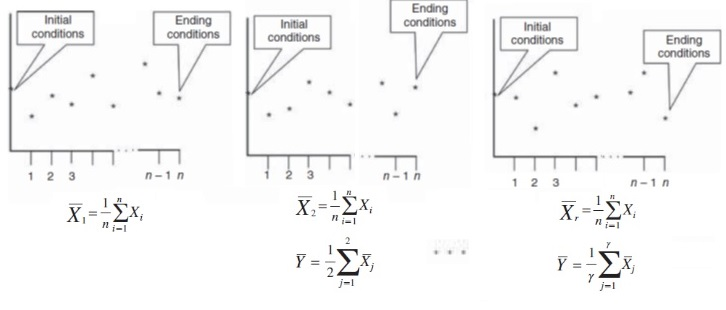
\includegraphics[width=11.5cm]{images/Statistics.jpg}
        %\caption{Caption}
        %\label{fig:my_label}
    \end{figure}
\end{frame}

\begin{frame}{Observaciones}
    \begin{itemize}
            \item Las observaciones pueden ser de dos tipos:
        \begin{itemize}
            \item \textbf{Tally}: representa una secuencia de datos que no persisten en el tiempo (tiempo en cola, número de entidades procesadas, si un cliente en particular esperó más de 10 minutos, etc.) 
            \item \textbf{Time-persistent}: representa una secuencia de valores que persisten durante un cierto tiempo, el valor se pondera por la cantidad de tiempo que persiste (promedio de entidades en cola, porcentaje de tiempo que hay cola, utilización del servidor, etc.)
        \end{itemize}
    \end{itemize}
\end{frame}
    
    \section[Horizonte finito]{Análisis de Simulación con horizonte finito}

%\begin{frame}{Análisis de Simulación con horizonte finito}
%    \begin{itemize}
%        \item Un modelo de simulación de horizonte finito puede analizarse con las metodologías estadísticas tradicionales, las cuales asumen un muestreo aleatorio, es decir, con variables aleatorias independientes e idénticamente distribuidas.
%        \item Para obtener una muestra aleatoria, se ejecuta la simulación comenzando con las mismas condiciones iniciales y asegurando que los números aleatorios usados dentro de cada réplica sean independientes. Cada réplica debe terminar también bajo las mismas condiciones.
%        \item Debe notarse que la independencia puede conseguirse en las estadísticas entre las réplicas. En tal caso se dice que las réplicas son independientes. Los datos dentro de la réplica pueden no ser independientes.
%    \end{itemize}
%\end{frame}

\begin{frame}{Análisis de Simulación con horizonte finito}
    El análisis estadístico en este caso se basa en tres requerimientos básicos:
    \begin{enumerate}
        \item Las observaciones son independientes.
        \item Las observaciones provienen de muestras con idéntica distribución.
        \item Las observaciones son extraidas de una distribución normal (o se tienen suficientes observaciones para recurrir al teorema del límite central).
    \end{enumerate}
\end{frame}

\begin{frame}{Análisis de Simulación con horizonte finito}
    \begin{itemize}
        \item Suponga que se tienen $n$ réplicas de una simulación. Sea $Y_{rj}$ la $j$-ésima observación de la réplica $r$ para $j=1,2,\dots,m_r$, donde $m_r$ es el número de observaciones en la réplica $r$, y $r=1,2,\dots,n$.
        \item El promedio muestral de cada réplica es:
    \[\overline{Y_r}=\frac{1}{m_r}\sum_{j=1}^{m_r}{Y_{rj}} \qquad \text{o} \qquad \overline{Y_r}=\frac{1}{T_E}\int_{0}^{T_E}{Y_r(t) dt}\]
        \item $\overline{Y_r}$ es el promedio muestral de las observaciones dentro de la réplica $r$, es una variable aleatoria que puede ser observada al final de la réplica; por lo tanto, $\overline{Y_r}$ para $r=1,2,\dots,n$, forma una muestra aleatoria.
    \end{itemize}
\end{frame}
    
\begin{frame}{Determinación del número de réplicas}
    \begin{itemize}
        \item El criterio clave de diseño para el experimento será el número de réplicas necesarias. %En otras palabras, se necesita determinar el tamaño de la muestra.
        \item El enfoque que se tomará es determinar la cantidad de muestras para que podamos tener una alta confianza en la estimación puntual.
        %\item Como el intervalo de confianza puede formar la base para la toma de decisiones, se puede utilizar el ancho medio del intervalo de confianza para determinar el tamaño muestral.
        \item La cantidad
        \[h=t_{\alpha/2,n-1}\frac{s}{\sqrt{n}}\]
        se llama \textit{ancho medio} del intervalo de confianza.
    \end{itemize}
\end{frame}    

    
\begin{frame}{Determinación del número de réplicas}
    \begin{itemize}
        \item Hay tres métodos para determinar el tamaño de la muestra:
        \begin{enumerate}
            \item Un método iterativo basado en la distribución $t$.
            \item Un método aproximado basado en la distribución normal.
            \item El método de la razón de ancho medio.
        \end{enumerate}
        \item Todos los métodos asumen que se cuenta con un conjunto de réplicas piloto $n_0$. %representativas de la población bajo estudio.
        %\item Cuando los datos no están normalmente distribuidos, se debe apelar al teorema de central para obtener resultados aproximados.
        %\item El supuesto de normalidad está típicamente justificado cuando las estadísticas entre réplicas se basan en promedios dentro de las réplicas.
    \end{itemize}
\end{frame}  

\begin{frame}{Determinación del número de réplicas}{Método iterativo con la distribución t}
    \begin{itemize}
        %\item El intervalo de confianza para un estimador puede servir como base para determinar el número de réplicas requeridas en la muestra.
        
        \item Se fija un error máximo, $\epsilon$, en el ancho medio, seleccionando un número de réplicas $n$ que satisfaga:
        \[h=t_{\alpha/2,n-1}\frac{s}{\sqrt{n}}\leq \epsilon\]
        \item Sin embargo, $t_{\alpha/2,n-1}$ depende de $n$, por lo tanto, la ecuación anterior es iterativa. 
        \item Se deben probar varios valores de $n$ hasta que se satisface la condición.
    \end{itemize}
\end{frame}

\begin{frame}{Determinación del número de réplicas}{Método aproximado basado en la distribución normal}
    \begin{itemize}
        %\item Alternativamente, el número de réplicas requeridas se puede aproximar usando la distribución normal.
        \item Resolviendo la ecuación anterior para $n$ se obtiene:
        \[n\geq \left(\frac{t_{\alpha/2,n-1} s}{\epsilon}\right)^2\]
        \item A medida que $n$ crece, $t_{\alpha/2,n-1}$ converge hacia el $100(1-\alpha/2)$ punto  porcentual de la distribución normal estándar $z_{\alpha/2}$.
        \item Lo cual arroja la siguiente aproximación:
        \[n\geq \left(\frac{z_{\alpha/2} s}{\epsilon}\right)^2\]
        \item Esta ecuación generalmente funciona bien para valores de $n$ grandes ($n>50$).
    \end{itemize}
\end{frame}

\begin{frame}{Determinación del número de réplicas}{Método aproximado basado en la distribución normal para proporciones}
    \begin{itemize}
        \item Si la medida de desempeño de interés es una proporción, se puede utilizar un método diferente. Un intervalo de confianza de $100\times(1-\alpha)\%$ para una proporción $p$ tiene la forma:
        \[\hat{p}\pm z_{\alpha/2} \sqrt{\frac{\hat{p}(1-\hat{p})}{n}}\]
        donde $\hat{p}$ es el estimador de $p$.
        \item A partir de esto, se puede determinar el número de réplicas mediante la siguiente ecuación:
        \[n=\left(\frac{z_{\alpha/2}}{\epsilon}\right)^2 \hat{p}(1-\hat{p})\]
        \item Una corrida piloto servirá para obtener el valor inicial del estimado $\hat{p}$.
    \end{itemize}
\end{frame}

%%%% EJERCICIO 3.4 pagina 82-108 de Rossetti

\begin{frame}{Determinación del número de réplicas}{Método de la razón de ancho medio}
    \begin{itemize}
        \item Sea $h_0$ el valor inicial del ancho medio de una corrida piloto: 
        \[h_0=t_{\alpha/2,n_0-1}\frac{s_0}{\sqrt{n_0}}\]
        \item Resolviendo para $n_0$ se obtiene:
        \[n_0=t^2_{\alpha/2,n_0-1}\frac{s^2_0}{h^2_0}\]
        \item En general, para cualquier $n$ se tiene:
        \[n=t^2_{\alpha/2,n-1}\frac{s^2}{h^2}\]
        \item Asumiendo que $t^2_{\alpha/2,n-1}\approx t_{\alpha/2,n_0-1}$ y que $s^2 \approx s^2_0$, a partir de la razón de $n_0$ a $n$ se obtiene que:
        \[n\cong n_0\frac{h^2_0}{h^2}=n_0\left(\frac{h_0}{h}\right)^2\]
        %que se conoce como la ecuación de la razón del ancho medio.
    \end{itemize}
\end{frame}


\begin{frame}{Determinación del número de réplicas}
    \begin{itemize}
        \item Para los métodos iterativo y de aproximación normal se requiere de un valor inicial para $s$. Este se puede obtener corriendo una muestra piloto (p.e. $n_0=10$).
        \item Cuando se ejecutan varias replicas en Arena, el reporte provee un intervalo de confianza de 95\% para las medidas de desempeño. 
        \item A partir del reporte del ancho medio puede obtenerse la desviación estándar como:%Arena no reporta la desviación estándar, sino directamente el ancho medio para un intervalo de confianza de 95\%.
         \[s_0=\frac{h_0\sqrt{n_0}}{t_{\alpha/2,n_0-1}}\]
        %\item Dado un valor de $s$, se puede definir un valor del error máximo y utilizar cualquiera de las fórmulas.
    \end{itemize}
\end{frame}

\begin{frame}{Determinación del número de réplicas}
    \begin{itemize}
        \item El error máximo, $\epsilon$, depende del problema y de la medida de desempeño específica que se esté observando. % Está bajo el control subjetivo del analista. El analista debe determinar un error razonable para la situación dada.       
        \item Debe considerarse que cuando se evalúa $n$, el error máximo $\epsilon$, está en el denominador elevado al cuadrado. %Esto implica que valor pequeños de $E$ resultarán en tamaños de muestra muy grandes.
        \item Si se tiene más de una medida de desempeño de interés, se puede usar cualquiera de las técnicas para determinar el número de réplicas necesarias para cada medida y utilizar la mayor entre todas. % If you have more than one performance measure of interest, you can use these sample size techniques for each of your performance measures and then use the maximum sample size required across the performance measures.
    \end{itemize}
\end{frame}

%%Sequential sampling

%%%% EJERCICIO 7.2 pagina 310-336 de Rossetti
    
    \section[Horizonte infinito]{Análisis de Simulación con horizonte infinito}

\begin{frame}{Análisis de Simulación con horizonte infinito}
    \begin{itemize}
        \item Existen dos métodos básicos para desarrollar simulaciones con estado estable:
        \begin{enumerate}
            \item Correr múltiples réplicas. 
            \item Correr una sola réplica muy larga. 
        \end{enumerate}
        \item Ambos métodos dependen del manejo de los aspectos no estacionarios de los datos.
    \end{itemize}
\end{frame}

\begin{frame}{Análisis de Simulación con horizonte infinito}

    \begin{itemize}
        \item Al analizar simulaciones con horizonte infinito, la principal dificultad es la naturaleza de los datos dentro de las réplicas.
        \item El análisis estadístico suele requerir:
        \begin{enumerate}
            \item Observaciones independientes.
            \item Observaciones tomadas de distribuciones idénticas.
            \item Observaciones extraídas de una distribución normal (o que haya suficientes observaciones para recurrir al teorema del límite central).
        \end{enumerate}
        \item Las salidas dentro de una réplica no satisfacen ninguna de esas condiciones; sin embargo, ciertos procedimientos pueden establecerse en la forma en que se toman los datos para asegurar que los supuestos no sean gravemente violados.
    \end{itemize}
\end{frame}

%Effect of initial conditions
\begin{frame}{Efecto de las condiciones iniciales}
    \begin{itemize}
        
        \item Sea $F_i(x|I)$ la distribución condicional acumulada de $X_i$ donde $I$ representa las condiciones utilizadas al iniciar la simulación en el tiempo 0. 
        \item Si $F_i(x|I)\rightarrow F(x)$ cuando $i \rightarrow \infty$, para cualquier $I$, entonces $F(x)$ se denomina la distribución de estado estable del proceso. 
        \item Las condiciones iniciales de una simulación, representan el estado del sistema cuando la simulación comienza.
    \end{itemize}
\end{frame}

\begin{frame}{Efecto de las condiciones iniciales}
    \begin{itemize}
        \item La dificultad al estimar el desempeño en estado estable, es que al menos que el sistema inicie utilizando la distribución de estado estable (la cual no se conoce), no hay forma de observar directamente la distribución de estado estable.
        \item La distribución $F_i(x|I)$ al comienzo de la simulación depende fuertemente de las condiciones iniciales.
        \item Si la distribución de estado estable existe, al correr una simulación suficientemente larga, los estimadores tienden a converger a las cantidades deseadas.
    \end{itemize}
\end{frame}

\begin{frame}{Efecto de las condiciones iniciales}{Estado transitorio y estable}
    \begin{figure}
        \centering
        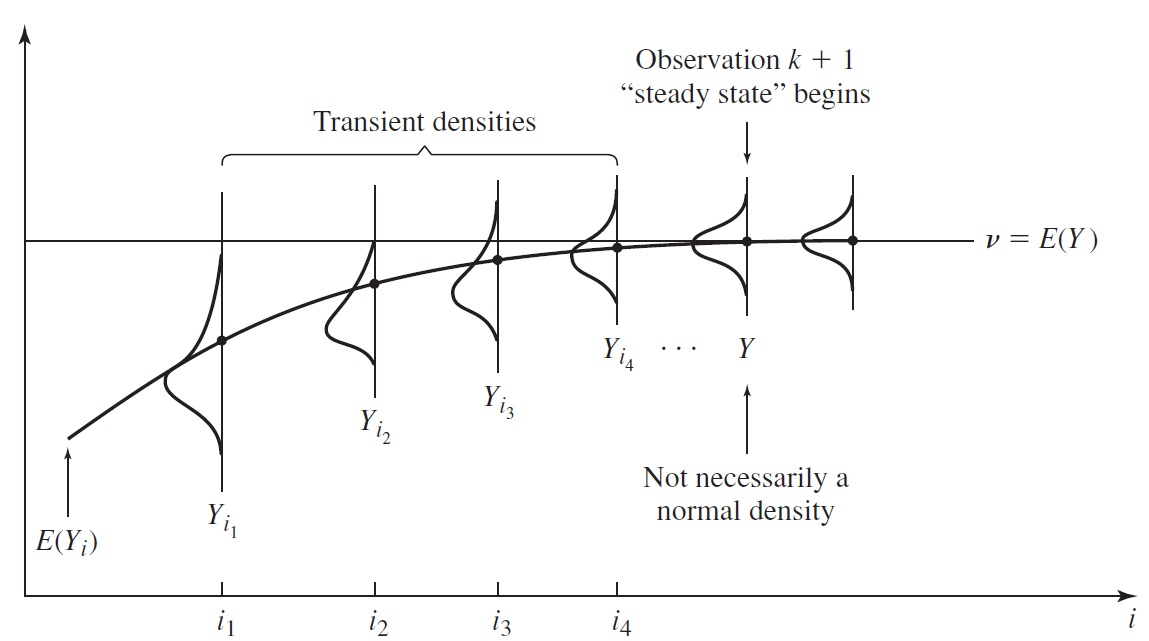
\includegraphics[width=8cm]{images/transientSteadyState.jpg}
        %\caption{Caption}
        \label{fig:TransientSteadyState}
    \end{figure}
\end{frame}

\begin{frame}{Efecto de las condiciones iniciales}
    \begin{itemize}
        \item Los estimadores de las medidas de desempeño en estado estable como los promedios muestrales tenderán a estar \textit{sesgados}. 
        \item Un estimador, $\hat{\theta}$, es un estimador \textit{insesgado} de un parámetro de interés $\theta$, si $E[\hat{\theta}]=\theta$.
        \item Si el estimador es sesgado, entonces la diferencia, $E[\hat{\theta}-\theta]$, se denomina el sesgo del estimador $\hat{\theta}$.
        \item El sesgo es una propiedad del estimador. Para estimar el sesgo de un estimador, se requiere contar con múltiples observaciones del estimador.
    \end{itemize}
\end{frame}

\begin{frame}{Periodo de calentamiento}
    \begin{itemize}
        \item Para mitigar el \textit{sesgo de inicialización}, aquel producido por la elección de unas condiciones iniciales específicas diferentes de $F(x)$, se puede emplear un método de simulación en dos fases.% conocido como \textit{periodo de calentamiento}.
        \item La estrategia consiste en encontrar un índice $d$, para el proceso de salida $X_i$, tal que $X_i; i=d+1, \dots$ tenga en esencia las mismas propiedades que la distribución en estado estable $F(x)$.
        \item Donde, $i=1,\dots, d$ es el \textit{periodo de calentamiento} del sistema y no se consideran para el cálculo de los estimadores. De esta forma, los estimadores de desempeño en estado estable se basan solo en $X_i;i=d+1, \dots$. 
    \end{itemize}
\end{frame}

\begin{frame}{Periodo de calentamiento}
    \begin{figure}
        \centering
        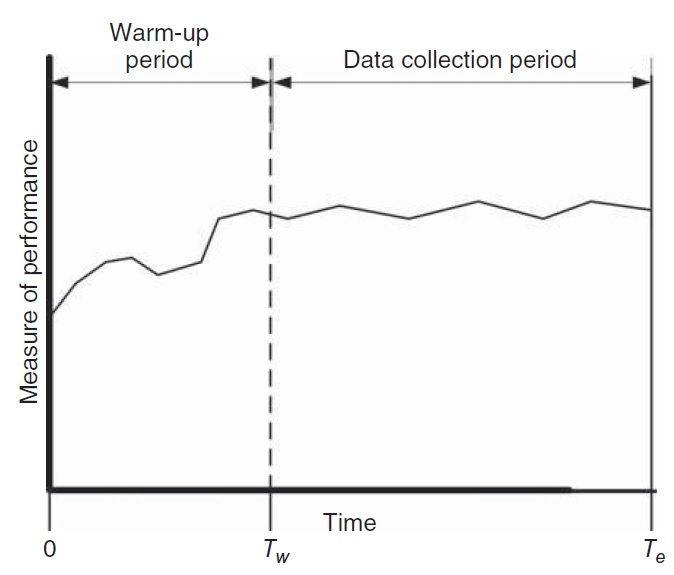
\includegraphics[width=8cm]{images/steady_state.jpg}
        %\caption{Caption}
        %\label{fig:my_label}
    \end{figure}
\end{frame}

\begin{frame}{Periodo de calentamiento}
    \begin{itemize}
        \item Varios métodos y políticas se han propuesto para determinar el periodo de calentamiento.
        \item Se explica a continuación un procedimiento gráfico:
            \begin{enumerate}
                \item Realice $n$ réplicas (se recomienda $n>5$).
                \item Sea $Y_{rj}$ la $j$-ésima observación en la réplica $r$, para $j=1,2,\dots,m_r$, donde $m_r$ es el número de observaciones en la réplica $r$.
                \item Calcule el promedio a través de cada réplica para cada $j=1,2,\dots,m$, donde $m=\min(m_r$, para $r=1,2,\dots,n$
                \[\bar{Y_{\cdot j}}=\frac{1}{n}\sum_{r=1}^{n}{Y_{rj}}\]
                \item Grafique $\bar{Y_{\cdot j}}$ para cada $j=1,2,\dots,m$.
                \item Evalúe visualmente dónde las gráficas comienzan a converger.
            \end{enumerate}
    \end{itemize}

\end{frame}

%Method of replication-deletion
\begin{frame}{Método de replicación-eliminación}
    \begin{itemize}
        \item Al realizar simulación de horizonte infinito especificando un periodo de calentamiento y haciendo múltiples réplicas, se emplea el \textit{método de replicación-eliminación}.
        \item Este método es muy utilizado en la práctica por la simplicidad del análisis después de que se ha determinado un periodo de calentamiento adecuado.
    \end{itemize}
\end{frame}

\begin{frame}{Método de replicación-eliminación}
    \begin{itemize}
        \item Al eliminar las estadísticas durante el periodo de calentamiento se reduce el sesgo de inicialización.
        \item Existe una compensación entre la variabilidad del estimador y el sesgo de inicialización. 
        \item Al eliminar parte de los datos, al variabilidad del estimador tiende a subir cuando el sesgo de inicialización disminuye.
    \end{itemize}
\end{frame}
    
\begin{frame}{Método de replicación-eliminación}
    \begin{itemize}
        \item En cada réplica, parte de los datos se desecha. Lo cual representa tiempo computacional que podría ser usado más eficientemente recolectando datos útiles.
        \item Las técnicas para determinar el periodo de calentamiento (como el procedimiento gráfico) requieren por lo general almacenar una cantidad significativa de datos.
    \end{itemize}
\end{frame}

\begin{frame}{Método de replicación-eliminación}
    \begin{itemize}
        \item Si se tienen múltiples medidas de desempeño, es posible que se requiera desarrollar un análisis del periodo de calentamiento por cada una, ya que cada medida de desempeño puede converger al estado estable a una tasa diferente.
        \item En tal caso, el periodo de calentamiento debe ser lo suficientemente grande como para cubrir todas las medidas de desempeño.
        \item De no especificarse un periodo de calentamiento suficientemente largo, es posible que esté agravando el problema del sesgo para las $n$ réplicas.
    \end{itemize}
\end{frame}

    %Batch means
\begin{frame}{Método de lotes equivalentes}
    \begin{itemize}
        \item En el método de los lotes equivalentes, solo se corre una réplica.
        \item Después de eliminar el periodo de calentamiento, el resto de la corrida es dividida en $k$ lotes, donde el promedio en cada lote representa una observación.
    \end{itemize}
\end{frame}

%As previously mentioned, the method of replication–deletion causes each replication to delete the initial portion of the run. As an alternative, you can make one long run and delete the initial portion only once. When analyzing an infinite-horizon simulation based on one long replication, a method is needed to address the correlation present in the within-replication data.

\begin{frame}{Método de lotes equivalentes}
    \begin{figure}
        \centering
        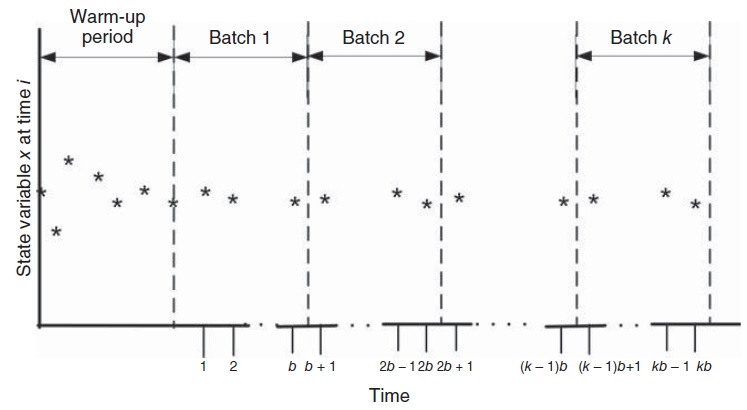
\includegraphics[width=10cm]{images/batch_means.jpg}
        %\caption{Caption}
        \label{fig:my_label}
    \end{figure}
\end{frame}

\begin{frame}{Método de lotes equivalentes}
    \begin{itemize}
        \item La ventaja de este método es que comprende una réplica muy larga, moderando el efecto de las condiciones iniciales.
        \item La principal desventaja es que las observaciones dentro de la réplica estás correlacionadas y a menos que se formen adecuadamente, los lotes pueden exhibir un fuerte grado de correlación.
    \end{itemize}
\end{frame}

\begin{frame}{Método de lotes equivalentes}
    \begin{itemize}
        \item El principal problema en este método es determinar el tamaño del lote o de forma alternativa el número de lotes a utilizar.
        \item Lotes más largos mejoran la independencia de las observaciones, pero reduce el número de lotes, resultando en una mayor varianza del estimador.
    \end{itemize}
\end{frame}
    
    %\section{Input Analyzer}

\begin{frame}{Input Analyzer}
    \begin{itemize}
        \item Input Analyzer es un complemento de Arena que puede emplearse para determinar la calidad del ajuste de datos de entrada a distintas funciones de distribución.
        \item Está disponible dentro de Arena en el menú Tools.
    \end{itemize}
\end{frame}

\begin{frame}{Preparación de archivos de datos}
    \begin{itemize}
        \item Se pueden crear en una hoja de cálculo o en un documento de texto.
        \begin{itemize}
            \item En una hoja de cálculo los datos se ingresan hacia abajo en una misma columna.
            \item En un documento de texto los datos deben separarse por: espacio, tabulaciones, guión corto.
        \end{itemize}
        \item Las extensiones del archivo pueden ser: .dst, .csv o .txt.
        \item Los datos no deben tener ningún tipo de encabezado.
        \item Se debe utilizar punto como separador decimal.
        \item No debe haber ningún tipo de caracter diferente a numéricos.
    \end{itemize}
\end{frame}

    \section*{Referencias} %You can remove this if you do not want to use it
        \begin{frame}{Referencias}
            \printbibliography
        \end{frame}
     
    \section{}   
        \begin{frame}{}
            \begin{figure}
                \centering
                
\includegraphics[width=6cm]{images/code.png}
                %\caption{Caption}
                %\label{fig:my_label}
            \end{figure}
        \end{frame}
      
\end{document}